% This file was created by matlab2tikz.
%
%The latest updates can be retrieved from
%  http://www.mathworks.com/matlabcentral/fileexchange/22022-matlab2tikz-matlab2tikz
%where you can also make suggestions and rate matlab2tikz.
%

\pgfplotsset{compat=newest}

\usetikzlibrary{calc}

%%% START MACRO FOR ANNOTATION OF TRIANGLE WITH SLOPE %%%.
\newcommand{\logLogSlopeTriangle}[5]
{
	% #1. Relative offset in x direction.
	% #2. Width in x direction, so xA-xB.
	% #3. Relative offset in y direction.
	% #4. Slope d(y)/d(log10(x)).
	% #5. Plot options.
	
	\pgfplotsextra
	{
		\pgfkeysgetvalue{/pgfplots/xmin}{\xmin}
		\pgfkeysgetvalue{/pgfplots/xmax}{\xmax}
		\pgfkeysgetvalue{/pgfplots/ymin}{\ymin}
		\pgfkeysgetvalue{/pgfplots/ymax}{\ymax}
		
		% Calculate auxilliary quantities, in relative sense.
		\pgfmathsetmacro{\xArel}{#1}
		\pgfmathsetmacro{\yArel}{#3}
		\pgfmathsetmacro{\xBrel}{#1-#2}
		\pgfmathsetmacro{\yBrel}{\yArel}
		\pgfmathsetmacro{\xCrel}{\xArel}
		%\pgfmathsetmacro{\yCrel}{ln(\yC/exp(\ymin))/ln(exp(\ymax)/exp(\ymin))} % REPLACE THIS EXPRESSION WITH AN EXPRESSION INDEPENDENT OF \yC TO PREVENT THE 'DIMENSION TOO LARGE' ERROR.
		
		\pgfmathsetmacro{\lnxB}{\xmin*(1-(#1-#2))+\xmax*(#1-#2)} % in [xmin,xmax].
		\pgfmathsetmacro{\lnxA}{\xmin*(1-#1)+\xmax*#1} % in [xmin,xmax].
		\pgfmathsetmacro{\lnyA}{\ymin*(1-#3)+\ymax*#3} % in [ymin,ymax].
		\pgfmathsetmacro{\lnyC}{\lnyA-#4*(\lnxA-\lnxB)}
		\pgfmathsetmacro{\yCrel}{\lnyC-\ymin)/(\ymax-\ymin)}
		
		% Define coordinates for \draw. MIND THE 'rel axis cs' as opposed to the 'axis cs'.
		\coordinate (A) at (rel axis cs:\xArel,\yArel);
		\coordinate (B) at (rel axis cs:\xBrel,\yBrel);
		\coordinate (C) at (rel axis cs:\xCrel,\yCrel);
		
		% Draw slope triangle.
		\draw[#5]   (A)-- node[pos=0.5,anchor=south] {\scriptsize 1}
		(B)-- 
		(C)-- node[pos=0.5,anchor=west] {\scriptsize #4}
		cycle;
	}
}

\newcommand{\logLogSlopeReverseTriangle}[5]
{
	% #1. Relative offset in x direction.
	% #2. Width in x direction, so xA-xB.
	% #3. Relative offset in y direction.
	% #4. Slope d(y)/d(log10(x)).
	% #5. Plot options.
	
	\pgfplotsextra
	{
		\pgfkeysgetvalue{/pgfplots/xmin}{\xmin}
		\pgfkeysgetvalue{/pgfplots/xmax}{\xmax}
		\pgfkeysgetvalue{/pgfplots/ymin}{\ymin}
		\pgfkeysgetvalue{/pgfplots/ymax}{\ymax}
		
		% Calculate auxilliary quantities, in relative sense.
		\pgfmathsetmacro{\xArel}{#1}
		\pgfmathsetmacro{\yArel}{#3}
		\pgfmathsetmacro{\xBrel}{#1+#2}
		\pgfmathsetmacro{\yBrel}{\yArel}
		\pgfmathsetmacro{\xCrel}{\xArel}
		%\pgfmathsetmacro{\yCrel}{ln(\yC/exp(\ymin))/ln(exp(\ymax)/exp(\ymin))} % REPLACE THIS EXPRESSION WITH AN EXPRESSION INDEPENDENT OF \yC TO PREVENT THE 'DIMENSION TOO LARGE' ERROR.
		
		\pgfmathsetmacro{\lnxB}{\xmin*(1-(#1-#2))+\xmax*(#1-#2)} % in [xmin,xmax].
		\pgfmathsetmacro{\lnxA}{\xmin*(1-#1)+\xmax*#1} % in [xmin,xmax].
		\pgfmathsetmacro{\lnyA}{\ymin*(1-#3)+\ymax*#3} % in [ymin,ymax].
		\pgfmathsetmacro{\lnyC}{\lnyA+#4*(\lnxA-\lnxB)}
		\pgfmathsetmacro{\yCrel}{\lnyC-\ymin)/(\ymax-\ymin)}
		
		% Define coordinates for \draw. MIND THE 'rel axis cs' as opposed to the 'axis cs'.
		\coordinate (A) at (rel axis cs:\xArel,\yArel);
		\coordinate (B) at (rel axis cs:\xBrel,\yBrel);
		\coordinate (C) at (rel axis cs:\xCrel,\yCrel);
		
		% Draw slope triangle.
		\draw[#5]   (A)-- node[pos=0.5,anchor=north] {\scriptsize 1}
		(B)-- 
		(C)-- node[pos=0.5,anchor=east] {\scriptsize #4}
		cycle;
	}
}
%%% END MACRO FOR ANNOTATION OF TRIANGLE WITH SLOPE %%%.


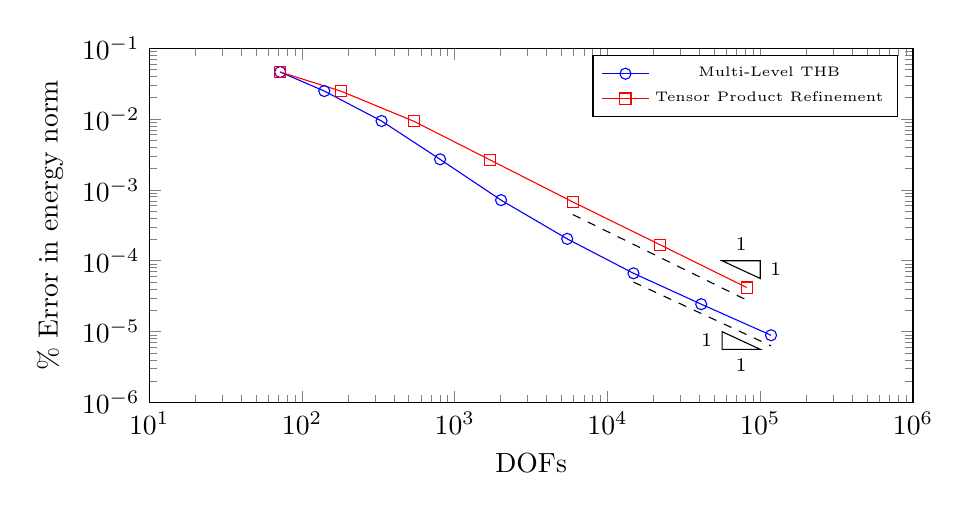
\begin{tikzpicture}

\begin{axis}[%
width=0.8\textwidth,
height=4.5cm,
at={(0in,0in)},
scale only axis,
xmode=log,
xmin=1e1,
xmax=1e6,
xminorticks=true,
ymode=log,
ymin=1e-06,
ymax=0.1,
yminorticks=true,
axis background/.style={fill=white},
ylabel=\% Error in energy norm,
xlabel=DOFs,
legend style={font=\tiny}
]
\addplot [color=blue,solid,mark=o,mark options={solid}]
table[row sep=crcr]{%
	72	0.046063507578358\\
	140	0.024827123605165\\
	332	0.009376820174183\\
	802	0.002701826251341\\
	2010	0.000717396099949\\
	5450	0.000203703205243\\
	14798	6.6550742906e-05\\
	41072	2.4392674541e-05\\
	117666	8.891058362e-06\\
};
\addplot [color=black,dashed,forget plot]
table[row sep=crcr]{%
%	72	0.0102891419539127\\
%	140	0.00529155871915513\\
%	332	0.00223138018277626\\
%	802	0.000923713492121843\\
%	2010	0.000368566278946128\\
%	5450	0.000135929948748939\\
	14798	5.00620503231327e-05\\
	41072	1.80370622487758e-05\\
	117666	6.29594122925669e-06\\
};

\addplot [color=red,solid,mark=square,mark options={solid}]
table[row sep=crcr]{%
	72	0.046063507578358\\
	180	0.02474434964774\\
	540	0.009296481785437\\
	1700	0.002654912173056\\
	5940	0.000674787313856\\
	22100	0.000168011560559\\
	81528	4.1901685859e-05\\
};
\addplot [color=black,dashed,forget plot]
table[row sep=crcr]{%
%	72	0.0481580925080468\\
%	180	0.0182327789805753\\
%	540	0.00568989611811802\\
%	1700	0.00168719727846886\\
	5940	0.000447948504665927\\
	22100	0.000111272004773931\\
	81528	2.78905145726206e-05\\
};

\legend{Multi-Level THB, Tensor Product Refinement}

{
\logLogSlopeReverseTriangle{0.75}{0.05}{0.15}{1}{black};
\logLogSlopeTriangle{0.8}{0.05}{0.4}{1}{black};
}
\end{axis}
\end{tikzpicture}%